\chapter{Time Complexity}\label{chap:ch10}

When discussing the efficiency of an algorithm, we aim to understand how it scales with input size, abstracting away details of specific hardware or programming environments. \textit{Theoretical} time complexity, commonly represented by Big-$\mathcal{O}$ notation (with a capital $\mathcal{O}$, not a zero), enables this abstraction by focusing on the dominant terms of an algorithm's behaviour as inputs grow large. This notation, also known as Landau's symbol, was introduced by the German number theorist Edmund Landau, with $\mathcal{O}$, standing for "order," capturing the growth rate of a function.

This chapter will introduce the tools needed to analyse algorithmic efficiency using Big-$\mathcal{O}$, Omega ($\Omega$), and Theta ($\Theta$) notation.\footnote{In practice, Big-$\mathcal{O}$ is often used informally as an umbrella term when discussing asymptotic analysis in a general sense, but it does not technically include $\Theta$ or $\Omega$. Each notation has its own specific use case in bounding the function's growth rate from different perspectives (upper, lower, and tight bounds), as we will see shortly.}

\section{Introduction to Complexity Analysis}\label{sec:ch10sec1}

For instance, analysing an algorithm might reveal that the time it takes to complete a problem of size $n$ is given by $T(n)=4 n^2-2 n+2$. By ignoring constants — since these vary with hardware and slower-growing terms - we simplify this to $T(n)=O\left(n^2\right)$, emphasizing the dominant term. This abstraction helps us understand complexity on large inputs, regardless of specific environments, making Big-$\mathcal{O}$ a powerful tool for comparing algorithms.

The two key components of this theoretical abstraction are:

\begin{enumerate}
    \item \textbf{Ignoring multiplicative constants:} Constants often depend on factors like processor speed or compiler optimisations, making them impractical for broad analysis.
    \item \textbf{Focusing on asymptotic behaviour:} We concentrate on the algorithm's behaviour with large inputs, as small cases typically run fast on any modern machine.
\end{enumerate}

However, in \textit{practical} time complexity, every term — including constants — plays a role. When running code on specific hardware with a known environment, those "negligible" constants in Big-$\mathcal{O}$ can become significant, especially for algorithms applied to small- and medium-sized data sets. So, while Big-$\mathcal{O}$ is crucial for high-level analysis and comparing algorithms, real-world complexity often requires looking at every term in the complexity expression. The following example illustrates this concept.

\begin{lstlisting}[style=pythonStyle, caption={Linear Search in Python}, label={lst:python_linear_search}]
    def linear_search(arr, target):
        for i in range(len(arr)):
            if arr[i] == target:
                return i
        return -1
\end{lstlisting} \newpage
    
% Use Java style for a Java code listing
\begin{lstlisting}[style=javaStyle, caption={Linear Search in Java}, label={lst:java_linear_search}]
    public static int linearSearch(int[] arr, int target) {
        for (int i = 0; i < arr.length; i++) {
            if (arr[i] == target) {
                return i;
            }
        }
        return -1;
    }
\end{lstlisting}

This code performs a linear search through a list, checking each element until it finds the target or reaches the end of the list. Here, the time complexity is $\mathcal{O}(n)$ in the worst case, as every element must be checked. For small lists, the difference may be negligible, but as the input size grows, the linear relationship between input size and runtime becomes evident.

When we ask "How efficient is an algorithm or piece of code?", we note that efficiency encompasses various resources, including:
\begin{itemize}
    \item CPU (time) usage
    \item Memory usage
    \item Disk usage
    \item Network usage
\end{itemize}

While all these resources are important, this chapter will primarily focus on time complexity, which concerns CPU usage.

\begin{enumerate}
    \item \textbf{Performance:} This refers to how much time, memory, disk space, or other resources are actually used when a program is run. Performance is influenced by factors such as the machine, compiler, runtime environment, and other implementation details in addition to the code itself.
    \item \textbf{Complexity:} Complexity, on the other hand, describes how the resource requirements of a program or algorithm scale with the size of the problem being solved. Complexity analysis focuses on the theoretical aspects of algorithm performance, characterizing how resource usage grows as input size increases.
\end{enumerate}

Complexity impacts performance, but performance alone does not provide a complete picture of an algorithm's efficiency in terms of scalability. Understanding both is crucial to evaluating how well an algorithm will perform in diverse realworld scenarios, especially as input sizes grow significantly.

\section{Growth of Functions}
In Section \ref{sec:ch10sec1}the introduction to this chapter we noted that Big-$\mathcal{O}$ notation focuses on the dominant term of an algorithm's time complexity, abstracting away constants and smaller terms. This simplification is based on the idea that, as input sizes grow large, the dominant term will dictate the algorithm's complexity. Consider the following Java code snippet:

\newpage

\begin{lstlisting}[style=javaStyle, caption={Java SumCalculator}, label={lst:java_f_function}]
    public static int f(int n) {
        int sum = 0;
        for (int i = 0; i < n; i++) {
            for (int j = 0; j < n; j++) {
                sum += (i + j) / 6;
            }
        }
        return sum;
    }
\end{lstlisting}

The code above is an implementation of the following expression:

\[
\operatorname{sum}=\sum_{i=0}^{n-1} \sum_{j=0}^{n-1} \frac{i+j}{6}
\]

Assuming $n$ is a non-negative integer, let $T(n)$ represent the CPU time taken by a typical laptop to execute the function\footnote{In Java, it's technically a method, not a function. In Java terminology, a function that belongs to a class (the function would probably belong to a class such as \inlinecode{public class SumCalculator}) is called a method. A function generally refers to a standalone block of code that can be invoked independently, which is typical in languages like C or Python.}  $f(n)$, with input $n$. Naturally, $T(n)$ can vary due to factors that we may not fully control, such as the specific Java compiler, the hardware specifications of the laptop, the operating system, and other applications running simultaneously. However, we can be certain of the structure of the loops: the outer loop runs $n$ times, and for each outer iteration, the inner loop also runs $n$ times, resulting in a total of $n^2$ iterations. 

Each iteration requires an approximate constant number of clock cycles, denoted \( c \), which can differ depending on the system. Instead of stating that "$T(n)$ is approximately \( cn^2 \) nanoseconds, for some constant \( c \) that varies across systems," we use Big-$\mathcal{O}$ notation to write \( T(n) = \mathcal{O}(n^2) \). This notation captures the idea that the CPU time grows at most quadratically with \( n \). To visualize this, consider a graph of \( T(n) \), which would generally appear parabolic with an approximate form of \( cn^2 \), where \( c > 0 \) is constant.

\begin{figure}[htbp]
    \centering
    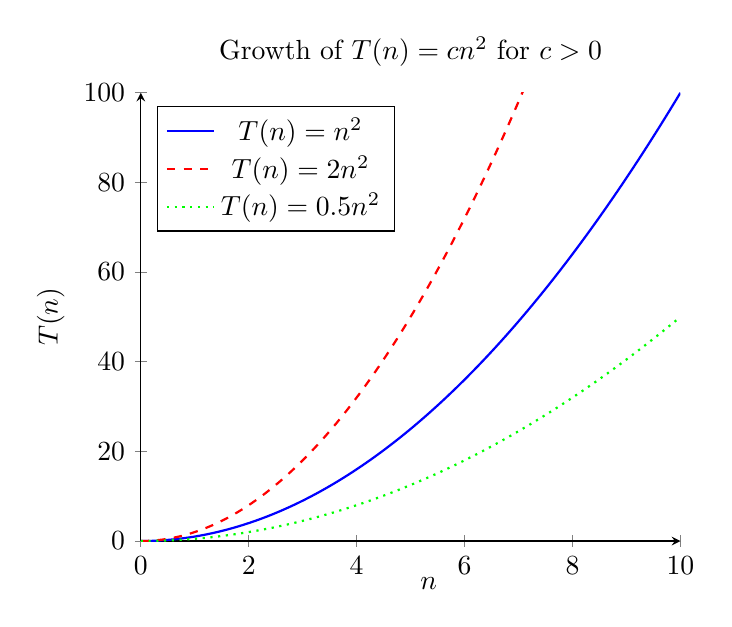
\begin{tikzpicture}
        \begin{axis}[
            domain=0:10,
            samples=100,
            axis lines=left,
            xlabel={$n$},
            ylabel={$T(n)$},
            ymin=0, ymax=100,
            xmin=0, xmax=10,
            xtick={0,2,4,6,8,10},
            ytick={0,20,40,60,80,100},
            xlabel style={right},
            ylabel style={above},
            legend pos=north west,
            title={Growth of $T(n) = cn^2$ for $c > 0$}
        ]
            \addplot[blue, thick] {x^2};
            \addlegendentry{$T(n) = n^2$}

            \addplot[red, thick, dashed] {2*x^2};
            \addlegendentry{$T(n) = 2n^2$}

            \addplot[green, thick, dotted] {0.5*x^2};
            \addlegendentry{$T(n) = 0.5n^2$}
        \end{axis}
    \end{tikzpicture}
    \caption{Graph of $T(n) = cn^2$ illustrating quadratic growth for different values of $c$}
    \label{fig:quadratic_growth}
\end{figure}

Big-$\mathcal{O}$ notation enables us to disregard constants, which often vary and lie beyond our control, yet do not affect the "family" or general growth rate classification of the function. For example, any potential $T(n)$ function in this case falls into the family of quadratic functions as illustrated in Figure \ref{fig:quadratic_growth}. Additionally, lower-order terms become insignificant for large $n$ as they can be bounded by a constant multiple of the dominant term. 

For instance, if $f(n) = 3.5n^2 + 4n + 36$, we observe that $f(n) \geq 3.5n^2$. Simultaneously,

\[
f(n) = 3.5n^2 + 4n + 36 \leq 3.5n^2 + 4n^2 + 36n^2 = 43.5n^2,
\]

which effectively "sandwiches" $f(n)$ between two quadratic functions, confirming that its growth is essentially quadratic.

\subsection*{Primitive Functions}
To understand how functions grow, let’s arrange some fundamental functions by their growth rates. We are looking for relationships of the form \( f(n) \leq g(n) \), but since we only care about behaviour with large inputs, these relationships hold only beyond some lower bound \( k \) for \( n \).

Starting with the basics, any constant function grows more slowly than a linear function, simply because a constant does not grow at all. For large enough values, a linear function grows slower than a quadratic, while a cubic function grows faster than a quadratic.

Exponentials are well known for their rapid growth. Consider the tale of a company that decided to reward an employee by doubling their bonus each day for a month. Although it started with a modest amount, the exponential increase quickly escalated, and by the end of the month, the bonus would have been astronomical. Realizing the unsustainable cost, the company swiftly revised the agreement to a fixed rate instead. Mathematically, this effect is clear: \( n^2 < 2^n \) for any integer \( n \geq 4 \). More generally, for any exponent \( k \), \( n^k < 2^n \) for sufficiently large \( n \).

Even more dramatically, factorial growth, represented by \( n! \), outpaces exponential growth for large \( n \). The reasoning is that \( 2^n \) consists of \( n \) factors of 2, while \( n! \) includes the first \( n \) integers as factors, most of which are larger than 2. Thus, \( n! \) eventually grows faster than \( 2^n \). 

To summarize, exponential growth is faster than any polynomial growth, and factorial growth surpasses both. Using \(1\) as our constant function, we can express these relationships as:

\[
1 \prec n \prec n^2 \prec n^3 \ldots \prec 2^n \prec n!
\]

The symbol \( \prec \) is used here because this ordering is not a standard algebraic inequality and only applies when \( n \) is sufficiently large.

For designing computer programs, only the first few of these growth rates are practical. Third-order polynomials can already grow too quickly for larger inputs, and exponential-time algorithms are only feasible for very small cases. Often, exponential algorithms are replaced by faster, approximate methods such as statistical sampling.

Now, let's consider functions with slower growth — these are the types of functions we aim for in efficient algorithms. Algorithms for searching in large datasets often have running times proportional to \( \log n \). If we plot \( \log n \) for values greater than 1, it shows slow but consistent growth, much slower than \( n \) itself.

\begin{figure}[htbp]
    \centering
    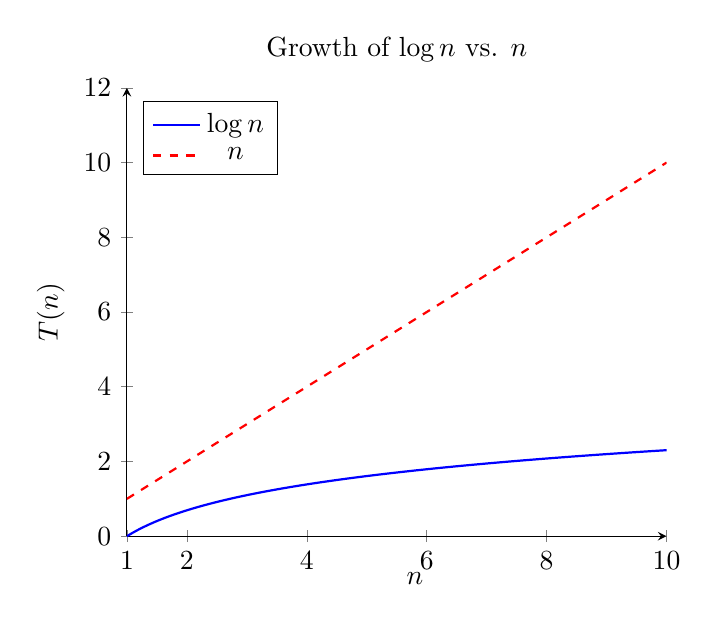
\begin{tikzpicture}
        \begin{axis}[
            domain=1:10,
            samples=100,
            axis lines=left,
            xlabel={$n$},
            ylabel={$T(n)$},
            ymin=0, ymax=12,
            xmin=1, xmax=10,
            xtick={1,2,4,6,8,10},
            ytick={0,2,4,6,8,10,12},
            xlabel style={right},
            ylabel style={above},
            legend pos=north west,
            title={Growth of $\log n$ vs. $n$}
        ]
            % Plot for log(n)
            \addplot[blue, thick] {ln(x)};
            \addlegendentry{$\log n$}

            % Plot for n
            \addplot[red, thick, dashed] {x};
            \addlegendentry{$n$}
        \end{axis}
    \end{tikzpicture}
    \caption{Graph comparing the growth rates of $\log n$ and $n$}
\end{figure}

Sorting algorithms, on the other hand, often have running times proportional to \( n \log n \). For large \( n \), we observe that \( 1 < \log n < n \), leading to \( n < n \log n < n^2 \). This order can be summarized as:

\[
1 \prec \log n \prec n \prec n \log n \prec n^2
\]

\begin{remark}
    When discussing $\log n$, we typically refer to the base-2 logarithm, as it is the most common in computer science and software engineering. However, the base of the logarithm does not affect the growth rate, as it only introduces a constant factor. For example, $\log_2 n$ and $\log_{10} n$ grow at the same rate, differing only by a constant multiple.
\end{remark}

\begin{table}[htbp]
    \centering
    \renewcommand{\arraystretch}{1.4}
    \begin{tabular}{|c|l|l|}
        \hline
        \textbf{Complexity} & \textbf{Growth Rate} & \textbf{Example Algorithms} \\
        \hline
        \( \mathcal{O}(1) \) & Constant & Accessing an array element \\
        \hline
        \( \mathcal{O}(\log n) \) & Logarithmic & Binary search \\
        \hline
        \( \mathcal{O}(n) \) & Linear & Linear search \\
        \hline
        \( \mathcal{O}(n \log n) \) & Linearithmic (or Log-Linear) & MergeSort, QuickSort, HeapSort \\
        \hline
        \( \mathcal{O}(n^2) \) & Quadratic & Bubble Sort, Selection Sort \\
        \hline
        \( \mathcal{O}(n^3) \) & Cubic & Matrix multiplication \\
        \hline
        \( \mathcal{O}(n^k) \) & Polynomial & Polynomial-time approximation algorithms \\
        \hline
        \( \mathcal{O}(c^n) \) & Exponential & Subset sum, brute force for combinatorial problems \\
        \hline
        \( \mathcal{O}(n!) \) & Factorial & Brute force for travelling salesperson \\
        \hline
        \( \mathcal{O}(n^n) \) & Super-exponential & Recursive algorithms with high branching factor \\
        \hline
    \end{tabular}
    \caption{Growth rates of common functions and example algorithms}
    \label{tab:growth_rates}
\end{table}


Table \ref{tab:growth_rates} summarizes the growth rates of common functions and supply some examples of algorithms that exhibit these growth rates and Figure \ref{fig:time_complexities} provides a visual representation of these growth rates. Memorizing the relative order of these common functions is valuable, as they will reappear frequently in this and other software engineering contexts.

\begin{figure}[htbp]
    \centering
    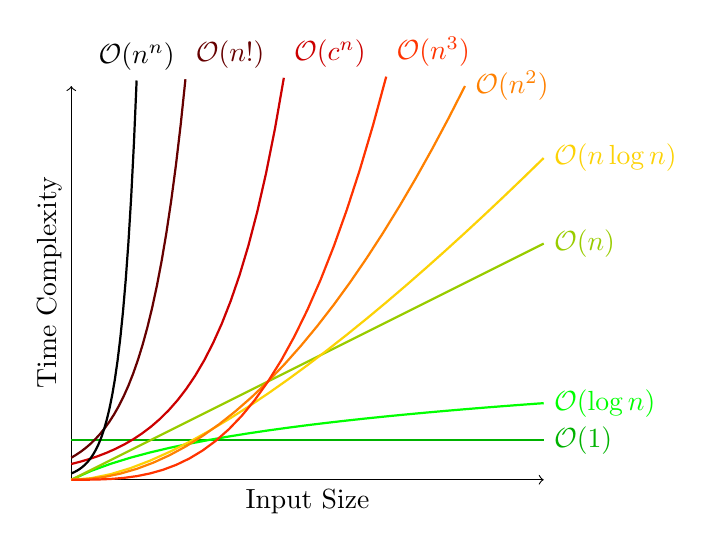
\begin{tikzpicture}
        % Draw axes
        \draw[->] (0,0) -- (0,5) node[midway, rotate = 90, anchor = south] {Time Complexity};
        \draw[->] (0,0) -- (6,0) node[below, midway] {Input Size};

        % Draw conceptual growth curves
        \draw[thick, green!70!black] plot [domain=0:6] (\x, {0.5}) node[right] {$\mathcal{O}(1)$};
        \draw[thick, green] plot [domain=0:6] (\x, {0.5*ln(\x+1)}) node[right] {$\mathcal{O}(\log n)$};
        \draw[thick, lime!80!black] plot [domain=0:6] (\x, {0.5*\x}) node[right] {$\mathcal{O}(n)$};
        \draw[thick, yellow!70!orange] plot [domain=0:6] (\x, {0.35*\x*ln(\x+1)}) node[right] {$\mathcal{O}(n \log n)$};
        \draw[thick, orange] plot [domain=0:5] (\x, {0.2*\x^2}) node[right] {$\mathcal{O}(n^2)$};
        \draw[thick, red!60!orange] plot [domain=0:4] (\x, {0.08*\x^3}) node[above right] {$\mathcal{O}(n^3)$};
        
        % Make O(2^n) and O(n!) much steeper
        \draw[thick, red!80!black] plot [domain=0:2.7] (\x, {0.2*exp(\x*1.2)}) node[above right] {$\mathcal{O}(c^n)$};
        \draw[thick, red!40!black] plot [domain=0:1.45] (\x, {0.28*exp(\x*2)}) node[above right] {$\mathcal{O}(n!)$};
        \draw[thick, black] plot [domain=0:0.83] (\x, {0.08*exp(\x*5)}) node[above] {$\mathcal{O}(n^n)$};

    \end{tikzpicture}
    \caption{Conceptual illustration of time complexities}
    \label{fig:time_complexities}
\end{figure}

In the next section, we introduce the framework for analysing algorithms using Big-$\mathcal{O}$, Omega ($\Omega$), and Theta ($\Theta$) notation, which allows us to describe the growth behaviour of functions more precisely. These notations correspond to the worst-case, best-case, and tight bounds of an algorithm's time complexity, respectively. Note that Theta ($\Theta$) notation is used when the upper and lower bounds of an algorithm's runtime are asymptotically the same, providing a precise description of the algorithm's complexity across different input sizes.


\section{Asymptotic Analysis}
In the analysis of algorithms, Big-$\mathcal{O}$, Omega ($\Omega$), and Theta ($\Theta$) notation each offer a unique perspective on an algorithm's efficiency, helping us understand how it will perform under different conditions. Whether we aim to determine the upper bound (worst-case scenario), lower bound (best-case scenario), or a tight bound, we can generally follow a systematic approach as follows:

\begin{enumerate}
    \item \textbf{Identify the Dominant Operations:} Focus on the operations that contribute most significantly to the running time, particularly those that grow the fastest as the input size increases.
    
    \item \textbf{Discard Constants and Lower-Order Terms:} For Big-$\mathcal{O}$ and $\Theta$ notation, ignore constant factors and lower-order terms to concentrate on the term that dictates the overall growth rate. For $\Omega$, ensure that you establish a lower bound that is still representative of the growth rate.
    
    \item \textbf{Express Complexity in Terms of the Input Size:} Write the complexity using $n$, the input size. If the runtime is proportional to the square of the input size, express it as $\mathcal{O}(n^2)$ if analysing an upper bound, $\Omega(n^2)$ if analysing a lower bound, or $\Theta(n^2)$ if establishing a tight bound.
\end{enumerate}


\begin{example}

Consider the function, $f(n)=4 n^3+3 n^2+2 n+10$. Let us determine the worst-case scenario, Big-$\mathcal{O}$, using the systematic approach outlined.
    \begin{enumerate}
        \item \textbf{Identify the Dominant Operations:}
        \begin{itemize}
            \item Look at each term in $f(n)=4 n^3+3 n^2+2 n+10$.
            The terms $4 n^3, 3 n^2, 2 n$, and 10 contribute differently to the running time.
            As $n$ grows, the $4 n^3$ term will dominate the growth of the function because $n^3$ grows faster than $n^2, n$, and constant terms. Therefore, we focus on $4 n^3$.
        \end{itemize}
        \item \textbf{Discard Constants:}
        \begin{itemize}
            \item Ignore the constant coefficient 4 in $4 n^3$, as Big-$\mathcal{O}$ notation only considers the asymptotic growth rate.
            We can disregard the lower-order terms $3 n^2, 2 n$, and 10 since they do not impact the asymptotic behaviour as $n$ becomes very large.
        \end{itemize}
        \item \textbf{Express Complexity in Terms of the Input Size $n$:}
        \begin{itemize}
            \item With the constants and lower-order terms removed, we are left with $n^3$.
            Since $4 n^3$ dominates the growth, we describe the complexity in terms of $n^3$ for all three notations

            \[
                f(n)=\mathcal{O}\left(n^3\right)
            \]
        \end{itemize}
    \end{enumerate}
\end{example}

Similar considerations apply to the best-case scenario, Omega ($\Omega$), and the tight bound, Theta ($\Theta$). We now introduce the three notations more in depth, starting with the tight bound notation, Theta ($\Theta$).

\subsection*{Theta (\texorpdfstring{$\Theta$}{Theta}) Notation}

Theta notation provides a \textit{tight bound}, indicating that the growth rate of a function is bounded both above and below by the same asymptotic expression. In other words, $\Theta$ notation is used when the upper and lower bounds of an algorithm’s runtime are the same, describing the algorithm’s complexity consistently across different input sizes.

Mathematically, $T(n) = \Theta(f(n))$ if there exist constants $c_1, c_2 > 0$ and $k \geq 0$ such that $c_1 \cdot f(n) \leq T(n) \leq c_2 \cdot f(n)$ for all $n \geq k$.

We can summarize this in the following definition:

\begin{definition}{Theta(\(\Theta\))}
    $f(n)$ is $\Theta(g(n))$ if there exist positive constants $c_1, c_2$, and $k$ such that for all $n \geq k$,
    \medskip
    \[
    c_1 \cdot g(n) \leq f(n) \leq c_2 \cdot g(n)
    \]
    \medskip
This means that $f(n)$ is asymptotically bounded both above and below by $g(n)$, meaning that $f(n)$ grows at the same rate as $g(n)$ as $n$ becomes sufficiently large.
\label{def:theta_notation}
\end{definition}

Note that by writing "$n$ becomes sufficiently large" we mean that the above inequalities do not have to hold for all $n \geq 0$, but rather for all $n \geq k$, for some constant $k \geq 0$. Sometimes we provide an exact value for $k$, and other times use the "sufficiently large" phrase when the value of $k$ is not important.

\begin{figure}[htbp]
    \centering
    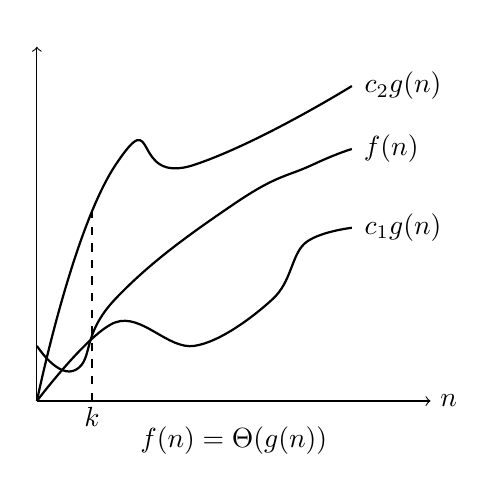
\begin{tikzpicture}
        % Axes
        \draw[->] (0,0) -- (5,0) node[right] {$n$};
        \draw[->] (0,0) -- (0,4.5) node[above] {};
        
        % Dashed line for n0
        \draw[dashed] (0.7,0) -- (0.7,2.5) node[below,yshift=-70pt] {$k$};

        % Plot for c1 * g(n) (lower bound) - Increase squiggles by lowering tension
        \draw[thick] plot[smooth, tension=0.6] coordinates {(0,0) (1,1) (2,0.7) (3, 1.3) (3.4, 2) (4,2.2)};
        \node at (4.65,2.2) {$c_1 g(n)$};

        % Plot for c2 * g(n) (upper bound) - Reduce squiggles by raising tension
        \draw[thick] plot[smooth, tension=1.0] coordinates {(0,0) (1,3) (2,3) (4,4)};
        \node at (4.65,4) {$c_2 g(n)$};

        % Plot for f(n) in between c1 g(n) and c2 g(n) - Fine-tuned squiggles by adjusting control points
        \draw[thick] plot[smooth, tension=0.8] coordinates {(0,0.7) (0.5,0.4) (1,1.3) (2.5,2.5) (3.5,3) (4,3.2)};
        \node at (4.5,3.2) {$f(n)$};
        
        % Label for Theta notation
        \node at (2.5,-0.5) {$f(n) = \Theta(g(n))$};
    \end{tikzpicture}
    \caption{Illustration of \(\Theta\)-notation with bounds on \( f(n) \) by \( c_1 g(n) \) and \( c_2 g(n) \)}
    \label{fig:theta_notation}
\end{figure}

Figure \ref{fig:theta_notation} illustrates the concept of $\Theta$ notation, showing how $f(n)$ is bounded both above and below by $c_1 g(n)$ and $c_2 g(n)$, respectively. The value of $k$ shown is the minimum possible value; any greater value would also work. Theta provides both an upper and lower bound for the running time of an algorithm and describes the asymptotic behaviour of the algorithm’s runtime, indicating that for sufficiently large inputs, the growth rate will stay within these bounds regardless of best-case or worst-case complexity. Or stated more succinctly:

\[
f(n)=\Theta(g(n)): \quad f \text { grows at the same rate as } g
\]

\begin{example}

    From the above discussion we have $f(n)=3.5 n^2+4 n+36=\Theta\left(n^2\right)$ since
    \[
    3.5 n^2 \leq f(n)=3.5 n^2+4 n+36 \leq 3.5 n^2+4 n^2+36 n^2=43.5 n^2,
    \]

is true for all $n \geq 1$. And so $f(n)=\Theta\left(n^2\right)$ by Definition \ref{def:theta_notation} , where $c_1=3.5$ and $c_2=43.5$.
\end{example}

The following properties hold for $\Theta$ notation:

\begin{itemize}
    \item If $f(n) = \Theta(g(n))$, then $g(n) = \Theta(f(n))$.
    \item If $f(n) = \Theta(g(n))$ and $g(n) = \Theta(h(n))$, then $f(n) = \Theta(h(n))$.
\end{itemize}

Also, the following proposition provides a convenient way to show that two functions have the same
order of growth.

\begin{proposition} \label{prop:limit_theorem}
    Let $f(n)$ and $g(n)$ be two nonnegative functions, and suppose there is a constant $c>0$ for which
    \medskip
    \[
    \lim _{n \rightarrow \infty} \frac{f(n)}{g(n)}=c
    \]
    \medskip
    Then $f(n)=\Theta(g(n))$. Also, if
    \medskip
    \[
    \lim _{n \rightarrow \infty} \frac{f(n)}{g(n)}
    \]
    \medskip
    exists but does \textbf{not} equal a positive constant, then $f(n) \neq \Theta(g(n))$.
\end{proposition}

\begin{example}
    Use Proposition \ref{prop:limit_theorem} to prove that if $f(n)=3 n^2+6 n+7$, then $f(n)=\Theta\left(n^2\right)$. In other words, $f(n)$ has quadratic growth.
\end{example}

\begin{solution}Let $g(n) = n^2$. According to Proposition \ref{prop:limit_theorem}, we need to compute the limit:
    
    \[
    \lim_{n \to \infty} \frac{f(n)}{g(n)} = \lim_{n \to \infty} \frac{3n^2 + 6n + 7}{n^2}.
    \]
    
    Dividing each term in the numerator by $n^2$, we get:
    \[
    \lim_{n \to \infty} \frac{3n^2}{n^2} + \frac{6n}{n^2} + \frac{7}{n^2} = \lim_{n \to \infty} \left( 3 + \frac{6}{n} + \frac{7}{n^2} \right).
    \]
    
    Now, as $n \to \infty$, the terms $\frac{6}{n}$ and $\frac{7}{n^2}$ approach $0$, so we have:
    \[
    \lim_{n \to \infty} \frac{f(n)}{g(n)} = 3.
    \]
    
    Since this limit is a positive constant ($c = 3 > 0$), by Proposition \ref{prop:limit_theorem}, it follows that $f(n) = \Theta(n^2)$.
    
    Thus, we have shown that $f(n) = 3n^2 + 6n + 7$ has quadratic growth, as required.
    \end{solution}
    

\subsection*{Upper and Lower Bound}

Suppose we define a function \( f(n) \) as follows:

\[
f(n) = 
\begin{cases} 
2n & \text{if } n \text{ is even} \\ 
3n^2 & \text{if } n \text{ is odd} 
\end{cases}
\]

What is the growth rate of \( f(n) \)? Unfortunately, we can't simply categorize \( f(n) \) as having either linear or quadratic growth. This is because the limits

\[
\lim_{n \rightarrow \infty} \frac{f(n)}{n}
\]

and

\[
\lim_{n \rightarrow \infty} \frac{f(n)}{n^2}
\]

do not exist, as \( f(n) \) continuously alternates between linear and quadratic behavior, switching from quadratic growth to linear growth and back. Therefore, the best we can do is to establish upper and lower bounds for \( f(n) \).

\textbf{For Big-$\mathcal{O}$: }\( f(n) = \mathcal{O}(g(n)) \) if \( f(n) \) does not grow faster than \( g(n) \). In other words, \( f(n) \leq c \cdot g(n) \) for some constant \( c > 0 \) and for all \( n \geq k \), where \( k \geq 0 \) is a constant.

\textbf{For Big-Omega:} \( f(n) = \Omega(g(n)) \) if \( f(n) \) grows at least as quickly as \( g(n) \). That is, \( f(n) \geq c \cdot g(n) \) for some constant \( c > 0 \) and for all \( n \geq k \), where \( k \geq 0 \) is a constant.

Using these definitions, we find that \( f(n) = \mathcal{O}(n^2) \) and \( f(n) = \Omega(n) \). We formalise these considerations in the following sections.

\subsection*{Big-\texorpdfstring{$\mathcal{O}$}{O} Notation}
Big-$\mathcal{O}$ notation provides an \textit{upper bound} on the growth rate of a function. It describes the worst-case scenario for an algorithm’s time complexity, indicating how the runtime or space requirements increase as the input size, $n$, grows. Big-$\mathcal{O}$ is particularly useful when comparing algorithms, as it allows us to focus on the most significant term that dictates complexity with large inputs.

\begin{definition}{Big-$\mathcal{O}$}
    $f(n)$ is $\mathcal{O}(g(n))$ if there exist positive constants $c$ and $k$ such that for all $n \geq k$,
    \medskip
    \[
    f(n) \leq c \cdot g(n)
    \]
    \medskip
    This means that $f(n)$ is asymptotically bounded above by $g(n)$, meaning that $f(n)$ grows at most as fast as $g(n)$ as $n$ becomes sufficiently large.
    \label{def:big_o_notation}
\end{definition}

The expression "$n$ becomes sufficiently large" implies that the inequality does not have to hold for all $n \geq 0$, but rather for all $n \geq k$, where $k$ is a constant. Often, we may not need the exact value of $k$, so we use "sufficiently large" when the exact value is unimportant.

\begin{figure}[htbp]
    \centering
    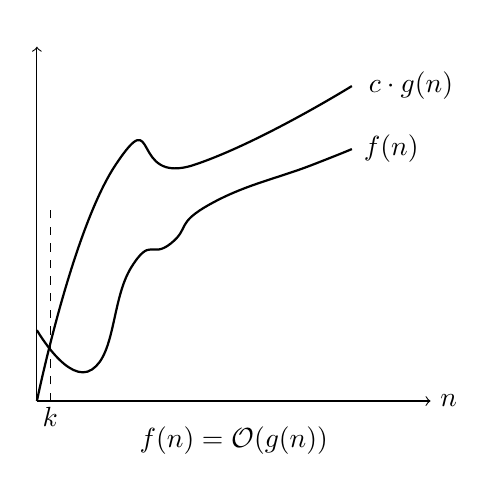
\begin{tikzpicture}
        % Axes
        \draw[->] (0,0) -- (5,0) node[right] {$n$};
        \draw[->] (0,0) -- (0,4.5) node[above] {};

        % Dashed line for n0
        \draw[dashed] (0.17,0) -- (0.17,02.5) node[below, yshift=-70pt] {$k$};

        % Plot for c * g(n) (upper bound)
        \draw[thick] plot[smooth, tension=1.0] coordinates {(0,0) (1,3) (2,3) (4,4)};
        \node at (4.75,4) {$c \cdot g(n)$};

        % Plot for f(n) below c * g(n)
        \draw[thick] plot[smooth, tension=0.9] coordinates {(0,0.9) (0.7,0.4) (1.2,1.7)  (1.7,2) (2.2,2.5) (3.5,3) (4,3.2)};
        \node at (4.5,3.2) {$f(n)$};
        
        % Label for Big O notation
        \node at (2.5,-0.5) {$f(n) = \mathcal{O}(g(n))$};
    \end{tikzpicture}
    \caption{Illustration of \(\mathcal{O}\)-notation with $f(n)$ bounded above by $c \cdot g(n)$.}
    \label{fig:big_o_notation}
\end{figure}

Figure \ref{fig:big_o_notation} illustrates the concept of Big-$\mathcal{O}$ notation, showing that $f(n)$ is bounded above by $c \cdot g(n)$. This notation provides an upper bound for the running time of an algorithm, describing the asymptotic behaviour of the algorithm’s runtime. It indicates that for sufficiently large inputs, the growth rate of $f(n)$ will not exceed this bound, regardless of the specific conditions or best-case complexity. Or stated more succinctly:

\[
f(n)=\mathcal{O}(g(n)): \quad f \text{ grows at most as fast as } g
\]


\begin{example}
    Using Definition \ref{def:big_o_notation}, show that $f(n)=3n^2+6n+7$ is $\mathcal{O}(n^2)$. In other words, $f(n)$ has at most quadratic growth.
\end{example}

\begin{solution}
    Let $g(n) = n^2$. We need to find constants $c > 0$ and $k$ such that $f(n) \leq c \cdot g(n)$ for all $n \geq k$.
    
    We can write:
    \[
    f(n) = 3n^2 + 6n + 7 \leq 3n^2 + 6n^2 + 7n^2 = 16n^2.
    \]
    Here, $c = 16$ and $k = 1$ work for the inequality, so we conclude $f(n) = \mathcal{O}(n^2)$.
\end{solution}

The following properties hold for $\mathcal{O}$ notation:
\begin{itemize}
    \item If $f(n) = \mathcal{O}(g(n))$ and $g(n) = \mathcal{O}(h(n))$, then $f(n) = \mathcal{O}(h(n))$.
    \item Constant functions are $\mathcal{O}(1)$, meaning their growth is bounded regardless of input size.
\end{itemize}

\subsection*{Omega (\texorpdfstring{$\Omega$}{Omega}) Notation}

Omega notation provides a \textit{lower bound} on the growth rate, describing the best-case scenario of an algorithm’s complexity. This notation is often used to indicate a guaranteed minimum time complexity, giving insight into how efficiently an algorithm can perform under ideal conditions. \newpage

\begin{definition}{Omega Notation}\label{def:omega_notation}
    $f(n)$ is $\Omega(g(n))$ if there exist positive constants $c$ and $k$ such that for all $n \geq k$,
    \medskip
    \[
    f(n) \geq c \cdot g(n)
    \]
    \medskip
    This means that $f(n)$ is asymptotically bounded below by $g(n)$, meaning that $f(n)$ grows at least as fast as $g(n)$ as $n$ becomes sufficiently large.
\end{definition}

The phrase "$n$ becomes sufficiently large" indicates that the above inequality does not need to hold for all $n \geq 0$, but only for $n \geq k$ for some constant $k$. 

\begin{figure}[htbp]
    \centering
    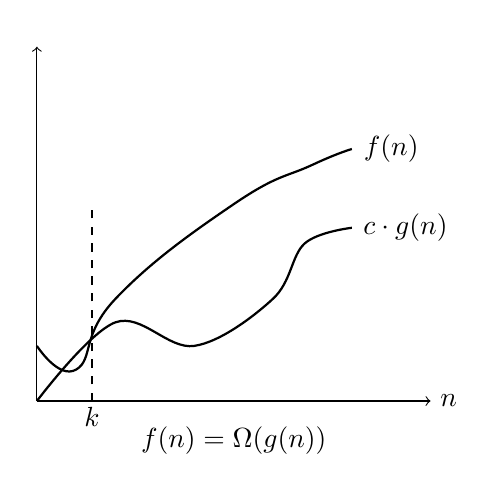
\begin{tikzpicture}
        % Axes
        \draw[->] (0,0) -- (5,0) node[right] {$n$};
        \draw[->] (0,0) -- (0,4.5) node[above] {};

        % Dashed line for n0
        \draw[dashed] (0.7,0) -- (0.7,2.5) node[below, yshift=-70pt] {$k$};

        % Plot for c * g(n) (lower bound)
        \draw[thick] plot[smooth, tension=0.6] coordinates {(0,0) (1,1) (2,0.7) (3, 1.3) (3.4, 2) (4,2.2)};
        \node at (4.68,2.2) {$c \cdot g(n)$};

        % Plot for f(n) above c * g(n)
        \draw[thick] plot[smooth, tension=0.8] coordinates {(0,0.7) (0.5,0.4) (1,1.3) (2.5,2.5) (3.5,3) (4,3.2)};
        \node at (4.5,3.2) {$f(n)$};
        
        % Label for Omega notation
        \node at (2.5,-0.5) {$f(n) = \Omega(g(n))$};
    \end{tikzpicture}
    \caption{Illustration of \(\Omega\)-notation showing $f(n)$ is asymptotically bounded below by $c \cdot g(n)$ for large values of $n$.}
    \label{fig:omega_notation}
\end{figure}

Figure \ref{fig:omega_notation} shows the concept of Omega notation, illustrating that $f(n)$ is bounded below by $c \cdot g(n)$. This notation provides a lower bound on the running time of an algorithm, describing the asymptotic growth rate of the algorithm's runtime in the best-case scenario. Or stated more succinctly:

\[
f(n)=\Omega(g(n)): \quad f \text{ grows at least as fast as } g
\]


\begin{example}
    Using Definition \ref{def:omega_notation}, show that $f(n)=3n^2+6n+7$ is $\Omega(n^2)$. In other words, $f(n)$ has at least quadratic growth.
\end{example}

\begin{solution}
    Let $g(n) = n^2$. We need to find constants $c > 0$ and $k$ such that $f(n) \geq c \cdot g(n)$ for all $n \geq k$.

    We can write:
    \[
    f(n) = 3n^2 + 6n + 7 \geq 3n^2.
    \]
    Here, $c = 3$ and $k = 1$ satisfy the inequality, so we conclude $f(n) = \Omega(n^2)$.
\end{solution}

The following properties hold for $\Omega$ notation:
\begin{itemize}
    \item If $f(n) = \Omega(g(n))$ and $g(n) = \Omega(h(n))$, then $f(n) = \Omega(h(n))$.
    \item Constant functions are $\Omega(1)$, meaning they have a lower bound that does not depend on input size.
\end{itemize}


In formal terms, $T(n) = \Omega(g(n))$ if there exist constants $c > 0$ and $k \geq 0$ such that $T(n) \geq c \cdot g(n)$ for all $n \geq k$.

For example, if a sorting algorithm always requires a minimum of $n \log n$ comparisons, we might say it has a time complexity of $\Omega(n \log n)$.

\begin{example}

    Suppose $f(n)$ is defined as follows.
    
    \[
    f(n)= \begin{cases}2 n^{2.1} \log ^3 n & \text { if } n \bmod 3=0 \\ 10 n^2 \log ^{50} n & \text { if } n \bmod 3=1 \\ 6 n^2 \log ^{30} n^{80} & \text { if } n \bmod 3=2\end{cases}
    \]
    
    
    Provide a Big-$\mathcal{O}$ upper bound and Big-$\Omega$ lower bound for $f(n)$.
    \end{example}
    
    \begin{solution}
        To find a Big-$\mathcal{O}$ upper bound and a Big-$\Omega$ lower bound for the function we examine each case and choose the term that grows the fastest as \( n \to \infty \) for the upper bound, and the term that grows the slowest for the lower bound.
        
        \textbf{Determine the Big-$\mathcal{O}$ Upper Bound}
        
        To find the Big-$\mathcal{O}$ upper bound, we look for the term with the highest growth rate as \( n \to \infty \). The term \( 2 n^{2.1} \log^3 n \) grows slightly faster than \( n^2 \) terms, as \( n^{2.1} \log^3 n \) will dominate \( n^2 \log^{50} n \) and \( n^2 \log^{30} n^{30} \) as \( n \) becomes large.
        
        Thus, a Big-$\mathcal{O}$ upper bound for \( f(n) \) is:
        \[
        f(n) = \mathcal{O}(n^{2.1} \log^3 n).
        \]
        
        \textbf{Determine the Big-$\Omega$ Lower Bound}
        
        For the Big-$\Omega$ lower bound, we look for the term with the slowest growth rate as \( n \to \infty \). The term \( n^2 \log^{50} n \) grows slower than \( n^{2.1} \log^3 n \), and it also has a slower growth rate than \( n^2 \log ^{30} n^{80} \).
        
        Therefore, a Big-$\Omega$ lower bound for \( f(n) \) is:
        \[
        f(n) = \Omega(n^2 \log^{50} n).
        \]
        
        In conclusion, we have:
        \[
        f(n) = \mathcal{O}(n^{2.1} \log^3 n) \quad \text{and} \quad f(n) = \Omega(n^2 \log^{50} n).
        \]\end{solution}

To summarise:
\begin{itemize}
    \item Big-$\mathcal{O}$ notation provides an upper bound, describing the \textit{worst-case} scenario.
    \item Omega ($\Omega$) notation gives a lower bound, capturing the \textit{best-case} scenario.
    \item Theta ($\Theta$) notation describes a tight bound, representing the algorithm’s \textit{consistent} complexity.
\end{itemize}

By understanding these notations, we gain a fuller perspective on an algorithm’s efficiency across different scenarios.

\section{Further Analysis}
Not all functions can be easily classified using Big-$\mathcal{O}$, Omega ($\Omega$), and Theta ($\Theta$) notation. In some cases, the growth rate of a function may not be easily determined, or the function may not fit neatly into one of these categories. In such cases, we can use additional tools to analyse the growth rate of functions more precisely.

\subsection*{Little-\texorpdfstring{$o$}{o} Notation}
Little-$o$ notation provides a \textit{strict upper bound} on the growth rate of a function. It describes a scenario where the function grows slower than another function, but not necessarily at the same rate. This notation is useful for indicating that an algorithm's time complexity is strictly less than a given function.

\begin{definition}{Little-$o$}\label{def:little_o_notation}
    $f(n)$ is $o(g(n))$ if for any positive constant $\epsilon > 0$, there exists a constant $k \geq 0$ such that for all $n \geq k$,
    \medskip
    \[
    f(n) < \epsilon \cdot g(n)
    \]
    \medskip
    This means that $f(n)$ grows strictly slower than $g(n)$ as $n$ becomes sufficiently large.
    
\end{definition}

The phrase "$n$ becomes sufficiently large" indicates that the above inequality does not need to hold for all $n \geq 0$, but only for $n \geq k$ for some constant $k$.

\begin{figure}[htbp]
    \centering
    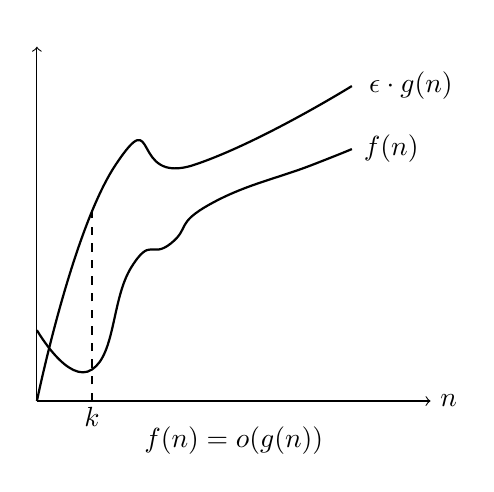
\begin{tikzpicture}
        % Axes
        \draw[->] (0,0) -- (5,0) node[right] {$n$};
        \draw[->] (0,0) -- (0,4.5) node[above] {};

        % Dashed line for n0
        \draw[dashed] (0.7,0) -- (0.7,2.5) node[below, yshift=-70pt] {$k$};

        % Plot for epsilon * g(n) (upper bound)
        \draw[thick] plot[smooth, tension=1.0] coordinates {(0,0) (1,3) (2,3) (4,4)};
        \node at (4.75,4) {$\epsilon \cdot g(n)$};

        % Plot for f(n) below epsilon * g(n)
        \draw[thick] plot[smooth, tension=0.9] coordinates {(0,0.9) (0.7,0.4) (1.2,1.7)  (1.7,2) (2.2,2.5) (3.5,3) (4,3.2)};
        \node at (4.5,3.2) {$f(n)$};
        
        % Label for Little o notation
        \node at (2.5,-0.5) {$f(n) = o(g(n))$};
    \end{tikzpicture}
    \caption{$o$-notation: $f(n)$ is strictly bounded above by $\epsilon \cdot g(n)$ for large $n$.}
    \label{fig:little_o_notation}
\end{figure}

Figure \ref{fig:little_o_notation} shows the concept of Little-$o$ notation, illustrating that $f(n)$ is strictly bounded above by $\epsilon \cdot g(n)$. This notation provides a strict upper bound on the running time of an algorithm, describing the asymptotic growth rate of the algorithm's runtime in a more precise manner. Or stated more succinctly:

\[
f(n)=o(g(n)): \quad f \text{ grows strictly slower than } g
\]

\begin{example}
    Using Definition \ref{def:little_o_notation}, show that $f(n)=3n^2+6n+7$ is $o(n^3)$. In other words, $f(n)$ grows strictly slower than $n^3$.
\end{example}

\begin{solution}
    Let $g(n) = n^3$. We need to show that for any positive constant $\epsilon > 0$, there exists a constant $k$ such that $f(n) < \epsilon \cdot g(n)$ for all $n \geq k$.

    We can write:
    \[
    f(n) = 3n^2 + 6n + 7 < \epsilon \cdot n^3
    \]
    for sufficiently large $n$. Dividing both sides by $n^3$, we get:
    \[
    \frac{f(n)}{n^3} = \frac{3n^2 + 6n + 7}{n^3} = \frac{3}{n} + \frac{6}{n^2} + \frac{7}{n^3}
    \]
    As $n \to \infty$, the right-hand side approaches $0$, which is less than any positive constant $\epsilon$. Therefore, $f(n) = o(n^3)$.
\end{solution}

This leads us to the following proposition

\begin{proposition} \label{prop:little_o_theorem}
    Let \( f(n) \) and \( g(n) \) be two nonnegative functions, and suppose
    \medskip
    \[
    \lim_{n \rightarrow \infty} \frac{f(n)}{g(n)} = 0
    \]
    \medskip
    Then \( f(n) = o(g(n)) \), meaning \( f(n) \) grows strictly slower than \( g(n) \) as \( n \to \infty \).
\end{proposition}

\begin{example}
    Use Proposition \ref{prop:little_o_theorem} to prove that if \( f(n) = 3n^2 + 6n + 7 \), then \( f(n) = o(n^3) \). In other words, \( f(n) \) grows strictly slower than \( n^3 \).

\end{example}

\begin{solution}
    
    Let \( g(n) = n^3 \). According to Proposition \ref{prop:little_o_theorem}, we need to compute the limit:
    
    \[
    \lim_{n \to \infty} \frac{f(n)}{g(n)} = \lim_{n \to \infty} \frac{3n^2 + 6n + 7}{n^3}
    \]
    
    Dividing each term in the numerator by \( n^3 \), we get:
    
    \[
    \lim_{n \to \infty} \frac{3n^2}{n^3} + \frac{6n}{n^3} + \frac{7}{n^3} = \lim_{n \to \infty} \left( \frac{3}{n} + \frac{6}{n^2} + \frac{7}{n^3} \right)
    \]
    
    Now, as \( n \to \infty \), the terms \( \frac{3}{n} \), \( \frac{6}{n^2} \), and \( \frac{7}{n^3} \) approach \( 0 \), so we have:
    
    \[
    \lim_{n \to \infty} \frac{f(n)}{g(n)} = 0
    \]
    
    Since this limit is \( 0 \), by Proposition \ref{prop:little_o_theorem}, it follows that \( f(n) = o(n^3) \).
    
    Thus, we have shown that \( f(n) = 3n^2 + 6n + 7 \) grows strictly slower than \( n^3 \), as required.
\end{solution}

The following properties hold for $o$ notation:
\begin{itemize}
    \item If $f(n) = o(g(n))$, then $g(n) \neq o(f(n))$.
    \item If $f(n) = o(g(n))$ and $g(n) = o(h(n))$, then $f(n) = o(h(n))$.
\end{itemize}

Little-$o$ notation provides a more precise way to describe the growth rate of functions, especially when the function grows strictly slower than another function. This notation is useful for indicating that an algorithm's time complexity is strictly less than a given function, providing a more detailed understanding of the algorithm's complexity.

\subsection*{Little-\texorpdfstring{$\omega$}{omega} Notation}
Little-$\omega$ notation provides a \textit{strict lower bound} on the growth rate of a function. It describes a scenario where the function grows faster than another function, but not necessarily at the same rate. This notation is useful for indicating that an algorithm's time complexity is strictly greater than a given function.

\begin{definition}{Little-$\omega$}\label{def:little_omega_notation}
    $f(n)$ is $\omega(g(n))$ if for any positive constant $\epsilon > 0$, there exists a constant $k \geq 0$ such that for all $n \geq k$,
    \medskip
    \[
    f(n) > \epsilon \cdot g(n)
    \]
    \medskip
    This means that $f(n)$ grows strictly faster than $g(n)$ as $n$ becomes sufficiently large.
\end{definition}

The phrase "$n$ becomes sufficiently large" indicates that the above inequality does not need to hold for all $n \geq 0$, but only for $n \geq k$ for some constant $k$.

\begin{figure}[htbp]
    \centering
    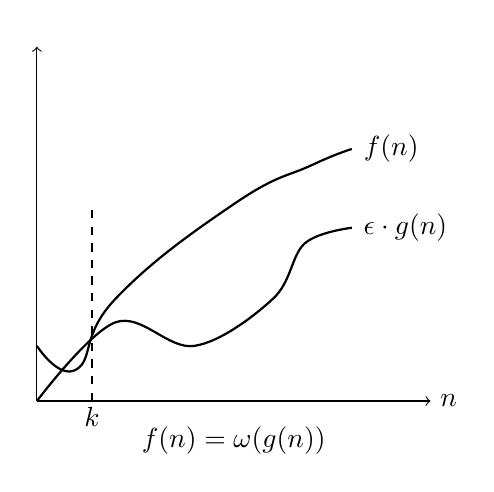
\begin{tikzpicture}
        % Axes
        \draw[->] (0,0) -- (5,0) node[right] {$n$};
        \draw[->] (0,0) -- (0,4.5) node[above] {};

        % Dashed line for n0
        \draw[dashed] (0.7,0) -- (0.7,2.5) node[below, yshift=-70pt] {$k$};

        % Plot for epsilon * g(n) (lower bound)
        \draw[thick] plot[smooth, tension=0.6] coordinates {(0,0) (1,1) (2,0.7) (3, 1.3) (3.4, 2) (4,2.2)};
        \node at (4.68,2.2) {$\epsilon \cdot g(n)$};

        % Plot for f(n) above epsilon * g(n)
        \draw[thick] plot[smooth, tension=0.8] coordinates {(0,0.7) (0.5,0.4) (1,1.3) (2.5,2.5) (3.5,3) (4,3.2)};
        \node at (4.5,3.2) {$f(n)$};
        
        % Label for Little omega notation
        \node at (2.5,-0.5) {$f(n) = \omega(g(n))$};
    \end{tikzpicture}
    \caption{$\omega$-notation: $f(n)$ is strictly bounded below by $\epsilon \cdot g(n)$ for large $n$.}
    \label{fig:little_omega_notation}
\end{figure}

Figure \ref{fig:little_omega_notation} shows the concept of Little-$\omega$ notation, illustrating that $f(n)$ is strictly bounded below by $\epsilon \cdot g(n)$. This notation provides a strict lower bound on the running time of an algorithm, describing the asymptotic growth rate of the algorithm's runtime in a more precise manner. Or stated more succinctly:

\[
f(n)=\omega(g(n)): \quad f \text{ grows strictly faster than } g
\]

\begin{example}
    Using Definition \ref{def:little_omega_notation}, show that $f(n)=n^3 + 6n + 7$ is $\omega(n^2)$. In other words, $f(n)$ grows strictly faster than $n^2$.
\end{example}

\begin{solution}
    Let $g(n) = n^2$. We need to show that for any positive constant $\epsilon > 0$, there exists a constant $k$ such that $f(n) > \epsilon \cdot g(n)$ for all $n \geq k$.

    We can write:
    \[
    f(n) = n^3 + 6n + 7 > \epsilon \cdot n^2
    \]
    for sufficiently large $n$. Dividing both sides by $n^2$, we get:
    \[
    \frac{f(n)}{n^2} = \frac{n^3 + 6n + 7}{n^2} = n + \frac{6}{n} + \frac{7}{n^2}
    \]
    As $n \to \infty$, the right-hand side approaches $n$, which is greater than any positive constant $\epsilon$. Therefore, $f(n) = \omega(n^2)$.
\end{solution}

This leads us to the following proposition:

\begin{proposition} \label{prop:little_omega_theorem}
    Let \( f(n) \) and \( g(n) \) be two nonnegative functions, and suppose
    \medskip
    \[
    \lim_{n \rightarrow \infty} \frac{f(n)}{g(n)} = \infty
    \]
    \medskip
    Then \( f(n) = \omega(g(n)) \), meaning \( f(n) \) grows strictly faster than \( g(n) \) as \( n \to \infty \).
\end{proposition}

\begin{example}
    Use Proposition \ref{prop:little_omega_theorem} to prove that if \( f(n) = n^3 + 6n + 7 \), then \( f(n) = \omega(n^2) \). In other words, \( f(n) \) grows strictly faster than \( n^2 \).
\end{example}

\begin{solution}
    Let \( g(n) = n^2 \). According to Proposition \ref{prop:little_omega_theorem}, we need to compute the limit:
    
    \[
    \lim_{n \to \infty} \frac{f(n)}{g(n)} = \lim_{n \to \infty} \frac{n^3 + 6n + 7}{n^2}
    \]
    
    Dividing each term in the numerator by \( n^2 \), we get:
    
    \[
    \lim_{n \to \infty} \frac{n^3}{n^2} + \frac{6n}{n^2} + \frac{7}{n^2} = \lim_{n \to \infty} \left( n + \frac{6}{n} + \frac{7}{n^2} \right)
    \]
    
    Now, as \( n \to \infty \), the term \( n \) approaches \( \infty \), so we have:
    
    \[
    \lim_{n \to \infty} \frac{f(n)}{g(n)} = \infty
    \]
    
    Since this limit is \( \infty \), by Proposition \ref{prop:little_omega_theorem}, it follows that \( f(n) = \omega(n^2) \).
    
    Thus, we have shown that \( f(n) = n^3 + 6n + 7 \) grows strictly faster than \( n^2 \), as required.
\end{solution}

The following properties hold for $\omega$ notation:
\begin{itemize}
    \item If $f(n) = \omega(g(n))$, then $g(n) \neq \omega(f(n))$.
    \item If $f(n) = \omega(g(n))$ and $g(n) = \omega(h(n))$, then $f(n) = \omega(h(n))$.
\end{itemize}


Little-$\omega$ notation provides a more precise way to describe the growth rate of functions, especially when the function grows strictly faster than another function. This notation is useful for indicating that an algorithm's time complexity is strictly greater than a given function, providing a more detailed understanding of the algorithm's complexity. 

\subsection*{Using Little-\texorpdfstring{$o$}{o} and Little-\texorpdfstring{$\omega$}{omega} to find \texorpdfstring{$\mathcal{O}$}{O} and \texorpdfstring{$\Omega$}{Omega}}
Little-$o$ and Little-$\omega$ notations can be used to provide more precise bounds when determining Big-$\mathcal{O}$ and $\Omega$ notations. They help in identifying whether a function grows strictly slower or faster than another function, which can be useful in asymptotic analysis.

\begin{example}
    Consider the function \( f(n) = n^2 + 3n + 2 \). We want to determine the Big-$\mathcal{O}$ and $\Omega$ notations.

    \begin{enumerate}
        \item \textbf{Big-$\mathcal{O}$ Notation:}
        
        To determine Big-$\mathcal{O}$, we consider the ratio \( \frac{f(n)}{g(n)} \), where \( g(n) = n^2 \). Using Proposition \ref{prop:big_o_theorem}, we compute the \(\limsup\)\footnote{The \(\limsup\) notation stands for the "limit superior" and considers the upper bound of the values of the ratio $\frac{f(n)}{g(n)}$ as $n$ grows. Unlike a regular limit, which may not exist if the function oscillates, \(\limsup\) will always exist for real-valued sequences and captures the maximum growth behaviour in the long run.}:
        \[
        \limsup_{n \to \infty} \frac{f(n)}{g(n)} = \limsup_{n \to \infty} \frac{n^2 + 3n + 2}{n^2} = \limsup_{n \to \infty} \left( 1 + \frac{3}{n} + \frac{2}{n^2} \right).
        \]
        As \( n \to \infty \), the terms \( \frac{3}{n} \) and \( \frac{2}{n^2} \) approach \( 0 \), so:
        \[
        \limsup_{n \to \infty} \frac{f(n)}{g(n)} = 1.
        \]
        Since this value is finite, we conclude that \( f(n) = \mathcal{O}(n^2) \).

        \item \textbf{Big-$\Omega$ Notation:}
        
        To determine Big-$\Omega$, we compute the \(\liminf\) of the same ratio\footnote{The \(\liminf\) notation stands for "limit inferior" and considers the lower bound of the values of the ratio $\frac{f(n)}{g(n)}$ as $n$ grows. Unlike a standard limit, which may fail to exist if the function oscillates, \(\liminf\) always exists for real-valued sequences. It captures the minimum long-term growth behaviour, highlighting the slowest rate at which $f(n)$ grows relative to $g(n)$ as $n$ becomes large.}:
        \[
        \liminf_{n \to \infty} \frac{f(n)}{g(n)} = \liminf_{n \to \infty} \frac{n^2 + 3n + 2}{n^2} = \liminf_{n \to \infty} \left( 1 + \frac{3}{n} + \frac{2}{n^2} \right).
        \]
        Again, as \( n \to \infty \), the terms \( \frac{3}{n} \) and \( \frac{2}{n^2} \) approach \( 0 \), so:
        \[
        \liminf_{n \to \infty} \frac{f(n)}{g(n)} = 1.
        \]
        Since this value is positive, we conclude that \( f(n) = \Omega(n^2) \).
    \end{enumerate}

    In conclusion, we have:
    \[
    f(n) = \mathcal{O}(n^2) \quad \text{and} \quad f(n) = \Omega(n^2).
    \]
\end{example}

        By using Little-$o$ and Little-$\omega$ notations, we can provide more precise bounds for Big-$\mathcal{O}$ and $\Omega$ notations, helping us better understand the growth rates of functions and the complexity of algorithms. But perhaps more importantly, we can use the concept of limits to determine Big-$\mathcal{O}$ and $\Omega$ notations from Little-$o$ and Little-$\omega$ notations.

        This leads us to the following propositions:

        \begin{proposition} \label{prop:big_o_theorem}
            Let \( f(n) \) and \( g(n) \) be two nonnegative functions. If
            \medskip
            \[
            \limsup_{n \rightarrow \infty} \frac{f(n)}{g(n)} < \infty
            \]
            \medskip
            then \( f(n) = \mathcal{O}(g(n)) \), meaning \( f(n) \) grows at most as fast as \( g(n) \) asymptotically.
        \end{proposition}
        
        And also:


        \begin{proposition} \label{prop:big_omega_theorem}
            Let \( f(n) \) and \( g(n) \) be two nonnegative functions. If
            \medskip
            \[
            \liminf_{n \rightarrow \infty} \frac{f(n)}{g(n)} > 0
            \]
            \medskip
            then \( f(n) = \Omega(g(n)) \), meaning \( f(n) \) grows at least as fast as \( g(n) \) asymptotically.
        \end{proposition}
        
        These propositions provide a more formal way to determine Big-$\mathcal{O}$ and $\Omega$ notations from Little-$o$ and Little-$\omega$ notations. By examining the limits of the ratios of functions, we can determine whether a function grows at most as fast or at least as fast as another function, providing a more rigorous analysis of growth rates.
            
            \begin{example}
            Use Proposition \ref{prop:big_omega_theorem} to prove that if \( f(n) = 3n^2 + 5n + 7 \), then \( f(n) = \Omega(n^2) \).
            \end{example}
            
            \begin{solution}
            Let \( g(n) = n^2 \). We need to compute the lower limit (lim inf) of \( \frac{f(n)}{g(n)} \) as \( n \) approaches infinity:
            
            \[
            \liminf_{n \to \infty} \frac{f(n)}{g(n)} = \liminf_{n \to \infty} \frac{3n^2 + 5n + 7}{n^2}.
            \]
            
            Dividing each term in the numerator by \( n^2 \), we have:
            \[
            = \liminf_{n \to \infty} \left( 3 + \frac{5}{n} + \frac{7}{n^2} \right).
            \]
            
            As \( n \to \infty \), the terms \( \frac{5}{n} \) and \( \frac{7}{n^2} \) approach \( 0 \). Thus, we obtain:
            \[
            \liminf_{n \to \infty} \frac{f(n)}{g(n)} = 3.
            \]
            
            Since this limit is a positive constant \( c = 3 > 0 \), by Proposition \ref{prop:big_omega_theorem}, it follows that \( f(n) = \Omega(n^2) \). This example demonstrates that \( f(n) = 3n^2 + 5n + 7 \) has quadratic growth in the lower bound sense. \end{solution}

            \begin{example}
                Determine if \( f(n) = 2n \sin(n) + 3n \) is \( \mathcal{O}(n) \) and \( \Omega(n) \) by using the limits as described in Proposition \ref{prop:big_o_theorem}. \end{example}
                
                \begin{solution}
                Let \( g(n) = n \). We will examine the behavior of \( \frac{f(n)}{g(n)} \) as \( n \to \infty \).
                
                First, express \( \frac{f(n)}{g(n)} \) as follows:
                \[
                \frac{f(n)}{g(n)} = \frac{2n \sin(n) + 3n}{n} = 2 \sin(n) + 3.
                \]
                
                Now, analyze the limit behavior as \( n \to \infty \):
                \[
                \lim_{n \to \infty} \frac{f(n)}{g(n)} = 2 \sin(n) + 3.
                \]
                
                Since \( \sin(n) \) oscillates between \( -1 \) and \( 1 \) as \( n \) grows, the expression \( 2 \sin(n) + 3 \) fluctuates between \( 1 \) and \( 5 \). Therefore, the simple limit \( \lim_{n \to \infty} \frac{f(n)}{g(n)} \) does not exist due to this oscillation.
                
                However, we can compute the \(\limsup\) and \(\liminf\) of \( \frac{f(n)}{g(n)} \):
                \[
                \limsup_{n \to \infty} \frac{f(n)}{g(n)} = 5 \quad \text{and} \quad \liminf_{n \to \infty} \frac{f(n)}{g(n)} = 1.
                \]
                
                Since \(\limsup\) is finite (\(5\)), we conclude that \( f(n) = \mathcal{O}(n) \) by Proposition \ref{prop:big_o_theorem}. Similarly, because \(\liminf\) is positive (\(1\)), we conclude that \( f(n) = \Omega(n) \) by Proposition \ref{prop:big_omega_theorem}.
                \end{solution}
                
                
                

        \subsection*{Using Limits to Determine Asymptotic Notations (An Informal Approach)}

        An informal but practical approach to determine Big-$\mathcal{O}$ and $\Omega$ involves examining the ratio \( \frac{f(n)}{g(n)} \) as \( n \to \infty \). We have already seen this approach in Propositions \ref{prop:limit_theorem}-\ref{prop:big_omega_theorem}. While not as rigorous as formal propositions, this method provides quick insights into growth rates.
        
        The following rules illustrate how limits can be applied to each notation:
       

        \begin{custombox}{Informal Limit Approach}
            \[
                \begin{array}{ll}
                \displaystyle \lim_{n \to \infty} \frac{f(n)}{g(n)} \neq \infty & \Rightarrow f(n) = \mathcal{O}(g(n)) \\[10pt]
                \displaystyle \lim_{n \to \infty} \frac{f(n)}{g(n)} \neq 0 & \Rightarrow f(n) = \Omega(g(n))
                \end{array}
                \]
                \medskip
                \textbf{Note:} This approach is an informal guideline and not a strict mathematical definition. There are cases where this limit-based method may not apply, but it often provides a convenient tool for determining asymptotic behavior.
        \end{custombox}
        
        These rules work as follows:
        \begin{itemize}
            \item \textbf{Big-\(\mathcal{O}\):} If the limit exists and is not infinity, then \( f(n) = \mathcal{O}(g(n)) \), meaning that \( f(n) \) does not grow faster than \( g(n) \).
            \item \textbf{Big-\(\Omega\):} If the limit exists and is non-zero, then \( f(n) = \Omega(g(n)) \), meaning that \( f(n) \) grows at least as fast as \( g(n) \).
        \end{itemize}
        
        \begin{example}
            Determine if $\sqrt{n} \cdot \log n=\mathcal{O}(n \log n)$ using the informal limit approach.
        \end{example}

        \begin{solution}
            We need to compute the limit of the ratio \( \frac{\sqrt{n} \cdot \log n}{n \log n} \) as \( n \to \infty \). Simplifying the expression, we get:
            
            \[
            \lim_{n \to \infty} \frac{\sqrt{n} \cdot \log n}{n \log n} = \lim_{n \to \infty} \frac{\sqrt{n}}{n} = \lim_{n \to \infty} \frac{1}{\sqrt{n}} = 0.
            \]
            
            Since the limit is finite, we conclude that \( \sqrt{n} \cdot \log n = \mathcal{O}(n \log n) \). We also notice that since the limit is 0, we can infer that \( \sqrt{n} \cdot \log n \neq \Omega(n \log n) \).
            
        \end{solution}

        \begin{solution}
            To determine if $\sqrt{n} \cdot \log n = \mathcal{O}(n \log n)$, we compute the following limit:
            
            \[
            \lim_{n \to \infty} \frac{\sqrt{n} \cdot \log n}{n \log n} = \lim_{n \to \infty} \frac{\sqrt{n}}{n} = \lim_{n \to \infty} \frac{1}{\sqrt{n}}.
            \]
        
            As $n \to \infty$, $\frac{1}{\sqrt{n}}$ approaches $0$. Since the limit is finite (not infinity), this result implies that $\sqrt{n} \cdot \log n = \mathcal{O}(n \log n)$.
        
            Therefore, we conclude that $\sqrt{n} \cdot \log n = \mathcal{O}(n \log n)$.
        \end{solution}
        
        The limit approach, while convenient, is not definitive. For some functions (e.g., oscillating functions), the formal definitions and propositions should be applied directly. This limit-based technique serves as a useful heuristic, particularly when the asymptotic growth is clear.
    
\subsection*{Comparing Notations}
We conclude this chapter by comparing the different asymptotic notations and their relationships:

\begin{enumerate}
    \item \( f(n) = \mathcal{O}(g(n)) \text{ and } f(n) = \Omega(g(n)) \Leftrightarrow f(n) = \Theta(g(n)) \)
    
    This relationship states that if \( f(n) \) is both asymptotically bounded above by \( g(n) \) (Big-\(\mathcal{O}\)) and bounded below by \( g(n) \) (Big-\(\Omega\)), then \( f(n) \) and \( g(n) \) grow at the same rate, denoted by \( \Theta(g(n)) \). In other words, \( f(n) \) grows neither faster nor slower than \( g(n) \) asymptotically, as \( n \to \infty \). \medskip

    \item \( f(n) = o(g(n)) \Rightarrow f(n) = \mathcal{O}(g(n)) \)
    
    If \( f(n) = o(g(n)) \), this means that \( f(n) \) grows strictly slower than \( g(n) \) as \( n \to \infty \). Therefore, \( f(n) \) is asymptotically bounded above by \( g(n) \) but does not grow as fast, justifying that \( f(n) = \mathcal{O}(g(n)) \).\medskip

    \item \( f(n) = \mathcal{O}(g(n)) \Leftrightarrow g(n) = \Omega(f(n)) \)
    
    This equivalence shows the symmetric nature of Big-\(\mathcal{O}\) and Big-\(\Omega\) notations. If \( f(n) \) is asymptotically bounded above by \( g(n) \) (meaning \( f(n) \) grows no faster than \( g(n) \)), then we can also say that \( g(n) \) grows at least as fast as \( f(n) \) (i.e., \( g(n) = \Omega(f(n)) \)). \medskip

    \item \( f(n) = \omega(g(n)) \Rightarrow f(n) = \Omega(g(n)) \)
    
    When \( f(n) = \omega(g(n)) \), this means that \( f(n) \) grows strictly faster than \( g(n) \) as \( n \to \infty \). Since \( f(n) \) is asymptotically larger, it follows that \( f(n) \) grows at least as fast as \( g(n) \), making \( f(n) = \Omega(g(n)) \) true. \medskip

    \item \( f(n) = o(g(n)) \Leftrightarrow g(n) = \omega(f(n)) \)
    
    This equivalence indicates the symmetric nature of Little-\(o\) and Little-\(\omega\) notations. If \( f(n) = o(g(n)) \), meaning \( f(n) \) grows strictly slower than \( g(n) \), then we can also say that \( g(n) \) grows strictly faster than \( f(n) \), or \( g(n) = \omega(f(n)) \). This relationship highlights the strict difference in their growth rates as \( n \to \infty \).
\end{enumerate}

In this chapter, we examined time complexity to evaluate algorithm efficiency. We introduced Big-$\mathcal{O}$, Omega ($\Omega$), and Theta ($\Theta$) notations as ways to establish upper, lower, and tight bounds on growth rates, which help us understand how runtime and space requirements scale with input size.

We highlighted the importance of ignoring constants and lower-order terms in asymptotic analysis, focusing instead on the dominant term. Additionally, we explored Little-$o$ and Little-$\omega$ notations for stricter upper and lower bounds, providing more precise insights into complexity.

Finally, we compared these notations and their key relationships, building a foundation for evaluating algorithm complexity both theoretically and practically — preparing us for hands-on time complexity analysis in the next chapter.
